%Made By Thomas Debelle
%Ajouté des Packages si nécessaires
\documentclass{report}
\usepackage[a4paper, total={6in, 9in}]{geometry}
\usepackage[utf8]{inputenc}
\usepackage[francais]{babel}
\usepackage{graphicx}
\usepackage{graphics}
\usepackage[T1]{fontenc}
\usepackage{amsmath}
\usepackage{hyperref}
\usepackage{amssymb}
\usepackage{listings}
\usepackage{xcolor}
\usepackage{array}
\usepackage{float}
\usepackage{amsfonts}
\usepackage{fancyhdr}
\usepackage{titlesec}
\usepackage{xparse}
\usepackage{wrapfig}

\hypersetup{
    colorlinks=true,
    linkcolor=black,
    filecolor=magenta,
    urlcolor=cyan,
    pdftitle={Overleaf Example},
    pdfpagemode=FullScreen,
    }
\begin{document}

%Si la mention "Juin 2023" est sur une autre page, changé le dernier VSPACE
\begin{titlepage}
    \begin{figure}
        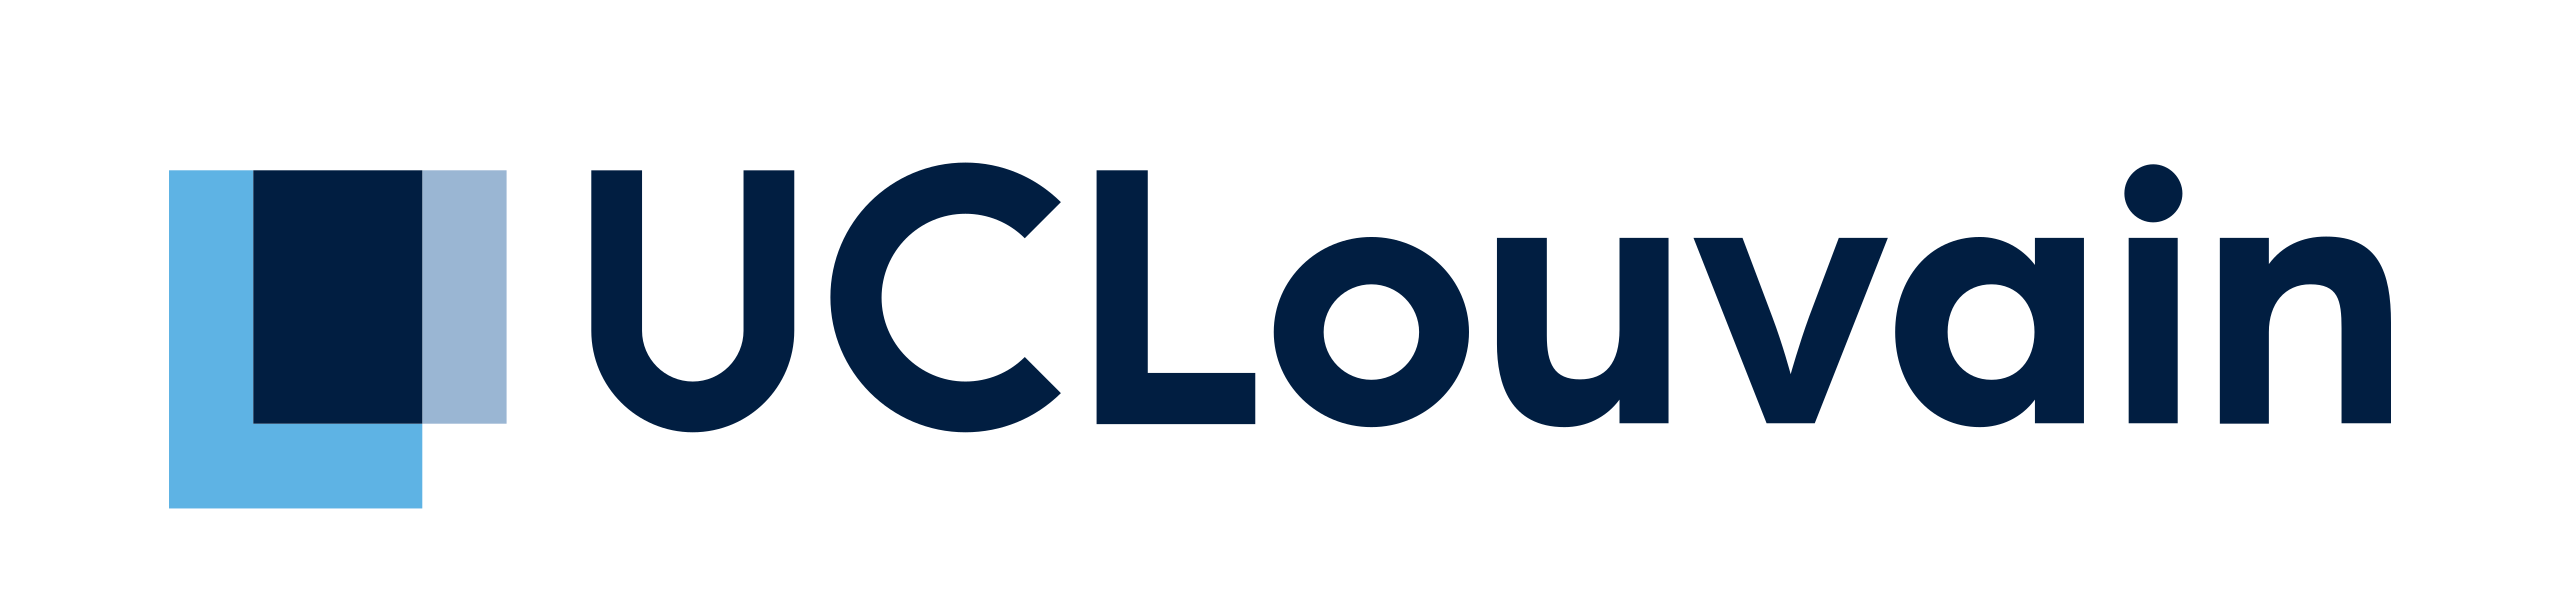
\includegraphics[height = 2cm]{UCL_Logo.png}
        \label{fig:my_label}
    \end{figure}

    \hspace*{100cm}
    \centering
    \vspace*{7cm}

    {\Huge \textbf{Résumé de LINFO1123}}\\
    \vspace*{0.25cm}
    compilation du \today\\
    \vspace*{0.25cm}
    \Large{Thomas Debelle}\\

    \vspace*{9.5cm} %Le dernier VSPACE
    {\Large Juin 2023}
\end{titlepage}

%_____NE PAS MODIFIER______
\tableofcontents
\newpage

\section*{Préface}

Bonjour à toi !\\

Cette synthèse recueille toutes les informations importantes données au cours, pendant les séances de tp et est amélioré grâce au note du Syllabus. Elle ne remplace pas le cours donc écoutez bien les conseils et potentielles astuces que les professeurs peuvent vous donner. Notre synthèse est plus une aide qui on l'espère vous sera à toutes et tous utiles.\\

Elle a été réalisée par toutes les personnes que tu vois mentionné. Si jamais cette synthèse a une faute, manque de précision, typo ou n'est pas à jour par rapport à la matière actuelle ou bien que tu veux simplement contribuer en y apportant ta connaissance ? Rien de plus simple ! Améliore la en te rendant \href{http://www.github.com/Tfloow/Q4_EPL}{ici} où tu trouveras toutes les infos pour mettre ce document à jour. (\textit{en plus tu auras ton nom en gros ici et sur la page du github})\\

Nous espérons que cette synthèse te sera utile d'une quelconque manière ! Bonne lecture et bonne étude.

%_______Vous pouvez modifier en-dessous_____
\chapter{Concepts}
Dans ce chapitre, on s'intéresse aux ensembles, cardinalité et équipotences de ces derniers
\section{Ensemble}
Un ensemble est un \textit{collection} d'objets, \textit{sans répétition}, ces derniers sont appelés \textit{éléments} de l'ensemble.
Donc un ensemble peut être des chiffres, des lettres, il peut être vide symbolisé par $void$ %à ajouter
On peut réaliser des opérations dessus, on peut déterminer des \textit{sous-ensembles d'ensemble} donc des ensembles issus d'ensemble.
On a également une notion s'appelant le \textit{complément} d'un ensemble dénoté $\tilde{A}$\\%trouver le bon charactère

\subsubsection{Langage}
Un \textit{langage} n'est autre qu'un mot ou bien un ensemble de caractères d'une taille fixée. Une chaine vide est écrite via le caractère "$\epsilon$".\\
On forme un langage via un \textit{alphabet} qui n'est autre qu'un ensemble de symboles, on le dénote "$\Sigma$". Tout langage est donc une suite de symbole issue de l'\textit{alphabet}.\\
$\Sigma^*$ correspond à l'ensemble des langages formés via l'alphabet.

\subsubsection{Relations}
Lorsque nous avons deux ensembles appelés \textit{A} et \textit{B}, on peut établir une relation appelé \textcolor{brown}{R} qui nous donne un sous-ensemble $AXB$ %trouver le symbole pour cross product
On peut représenter la relation par une table.

\subsubsection{Fonctions}
Lorsque nous avons deux ensembles appelés \textit{A} et \textit{B}, on peut avoir ce qu'on appelle une \textit{fonction} \textcolor{brown}{F}. C'est une relation tel que:
\begin{equation}
\exists a \in A : \exists b \in B :\quad <a,b> \quad \in f
\end{equation}
Il n'existe pas plus d'un b pour un a. Si pour un a il n'existe pas de b, on dit que $f(a)$ est indéfini et donc $f(a) = \perp$ ou \textit{bottom}.

\subsubsection{Propriétés des fonctions}
\begin{itemize}
\item un \textcolor{brown}{domaine de fonction} ou dom(f) $= {a \in A | f(a) \neq \perp}$
\item une \textcolor{brown}{image de fonciton} ou image(f) $= b \in B | \exists a \in A: b = f(a)$
\item f est dit \textcolor{brown}{fonction totale} si dom(f) $= A$
\item f est dit \textcolor{brown}{fonction partielle} si dom(f) $\in A$ % trouver le symbole pour include
\item f est \textcolor{brown}{surjectif} ssi image(f) = B autrement dit, tout élement est associé à minimum 1 élément dans B.
\item f est \textcolor{brown}{injectif} ssi $\forall a, a' \in A: a \neq a' \Rightarrow f(a)\neq f(a')$ autrement dit on ne fait correspondre qu'au plus un élément de A dans B.
\item f est \textcolor{brown}{bijectif} s'il combine \textit{surjectif} et \textit{injectif}
\end{itemize}

Intéressons nous aux \textcolor{red}{extensions} qui est le fait de rajouter une fonction qui ne définit un élément de B pas encore défini.
\begin{equation}
\forall x \in A : g(x) \neq \perp \Rightarrow f(x) = g(x)
\end{equation}	
f à la même valeur que g partout où g est défini.

\subsubsection{Définition d'une fonction}
Comme dit précédemment, une fonction est défini par sa table. On va souvent utiliser une description de la table qui permet que celle-ci soit clair et bien défini. De plus, on a pas besoin de savoir comment calculer ceci.\\
On peut également définir une table via une fonction ou un algorithme.

\section{Ensemble énumérable}
On dit que 2 ensembles ont le même cardinal (\textit{A} et \textit{B}) ssi il existe une bijection entre ces 2 ensembles. Donc chaque élément de \textit{A} correspond à un élément de \textit{B}.\\

On dit d'un ensemble qu'il est dénombrable ssi il est \textcolor{red}{fini} ou il existe une \textcolor{red}{bijection} entre l'ensemble $\mathbb{N}$ et cet ensemble.

\subsubsection{Exemples}
\begin{itemize}
\item L'ensemble $\mathbb{Z}$
\item L'ensemble des nombres pairs
\item Des paires d'entiers
\item L'ensemble des programmes Java
\end{itemize}

\subsubsection{Propriétés}
Tout sous-ensemble d'ensemble énumérable est \textit{énumérable}. L'union et l'intersection d'ensembles énumérables est \textit{énumérable}.\\

En s'intéressant à l'ensemble des programmes informatiques, on se rend compte que c'est une \textit{ensemble énumérable infini}. De plus, les programmes informatiques ne considèrent que des choses \textit{énumérables}.

\section{Cantor}
Le théorème de \textit{Cantor} nous dit que l'ensemble des nombres entre 0 et 1 compris est \textit{non énumérable}.
\begin{equation}
E = {x \in \mathbb{R} | 0 < x \le 1}
\end{equation}

\subsubsection{Preuve}
Pour prouver cela, on va réaliser une table et on va réaliser une \textit{diagonalisation de Cantor}.
\begin{center}
\begin{tabular}{|c||c|c|c|c|c|}
	\hline
	 & chiffre 1 & chiffre 2 & ... & chiffre $k+1$ & ...\\
	 \hline
	 $x_0$ & \textcolor{red}{$x_{00}$} & $x_{01}$ & ... & $x_{0k}$ & ...\\
	 \hline
	 $x_1$ & $x_{10}$ & \textcolor{red}{$x_{11}$} & ... & $x_{1k}$ & ...\\
	 \hline
	 ...& ... & ... & ... & ... & ...\\
	 \hline
	 $x_k$ & $x_{k0}$ & $x_{k1}$ & ... & \textcolor{red}{$x_{kk}$} & ...\\
	\hline
	 ...& ... & ... & ... & ... & ...\\
	\hline
\end{tabular}
\end{center}
Ensuite, on va définir notre nombre de la diagonale qui vaut $d = 0.x_{00}x_{11}...x_{kk}$. De cet valeur, on va créer une valeur $d'$ qui a comme propriété $x_{kk} \neq x'_{kk} \forall k$.\\
Mais, on doit stocker notre valeur $d'$ dans la table. On la stock à $p$ ce qui donne $d' = 0.x'_{p0}x'_{p1}... \textcolor{red}{x'_{pp}}$ mais à cause de la construction de $d = 0.x_{00}x_{11}...\textcolor{red}{x_{pp}}$. Par construction, $x'_{pp} \neq x_{pp}$ mais cela ne peut être respecté. Donc, \textbf{il n'y a pas} de \textit{bijection} des $\mathbb{N}$ vers cet ensemble. Donc cet ensemble est \textit{non énumérable}.

\subsubsection{Autre ensemble non énumérable}
\begin{itemize}
\item L'ensemble des $\mathbb{R}$.
\item L'ensemble des sous-ensemble de $\mathbb{N}$.
\item L'ensemble des chaines infinies de caractères d'un alphabet fini.
\item L'ensemble des \textit{fonctions} de $\mathbb{N}$ dans $\mathbb{N}$.
\end{itemize}
Chose intéressante à noter, comme on a une infinité non énumérable de fonctions $\mathbb{N}$ dans $\mathbb{N}$ et un nombre de programme informatique \textit{infini énumérable}. On ne peut résoudre tous les problèmes informatiques donc.

\chapter{Programmes calculables}
\section{Les algorithmes}
Un algorithme est un ensemble \textit{d'instructions} qui a pour but de produire un résultat. Donc un algorithme n'est \textcolor{red}{pas une fonction}. Il \textit{calcule} une fonction. Un algorithme n'est pas forcément un \textit{programme}, il peut être un \textit{organigramme}. C'est un \textit{ensemble fini d'instructions}. C'est une sorte de \textit{calculateur}. Ici, on va considérer nos algorithmes comme \textit{n'ayant pas de limite} de:
\begin{itemize}
\item Taille de données
\item Taille d'instructions
\item Taille de la mémoire, mais on a une utilisation finie.
\end{itemize}

\subsection{Calculabilité}
Avant de continuer, il faut définir la \textit{calculabilité} des algorithmes car sans \textit{formalisme}, les algorithmes sont non rigoureux, non exploitables.\\

Ici, on base cette notion sur celle des \textit{programmes informatiques}. (plus intuitif).
Ainsi, on possède \textbf{2 univers} celui des \textit{programmes informatiques} et celui des \textit{problèmes}. Pour être plus précis, on se base sur le \textcolor{brown}{langage Java} et on se limite au fonction $\mathbb{N} \rightarrow \mathbb{N}$. Ainsi pour les fonctions, on aura \textbf{1 entrée} et \textbf{1 sortie}. (on peut également généraliser ceci en disant que $\mathbb{N}^n \rightarrow \mathbb{N}$)

\section{Fonction calculable}
Une fonction est dite \textit{calculable} s'il existe un \textit{programme Java} recevant \textbf{1 donnée} étant un nombre $\in \mathbb{N}$ et la fonction va nous retourner la \textit{valeur} de $f(x)$ \textit{si} elle est défini.\\
Si le programme \textit{ne se termine pas} donc pas défini ou erreur d'exécution on dit que $f(x) = \perp$. On définit bien la notion de calculabilité sur \textit{l'existence d'un programme}. on a 2 types de fonctions
\begin{enumerate}
\item Fonction \textit{partielle} calculable: on a \textit{parfois} un résultat
\item Fonction \textit{totale} calculable: on peut \textit{toujours} calculé quelque chose.
\end{enumerate}

\subsection{Ensemble récursif}
Maintenant, on va essayer de déterminer la calculabilité sur \textit{un ensemble de fonctions}.
Le principe de décision de \textit{calculabilité} est le principe dit \textit{récursif}.\\
\textbf{A} est \textcolor{red}{récursif} si il existe un programme \textit{Java} qui recevant n'importe quelle donnée sous forme d'un $\mathbb{N}$ fourni comme résultat:
\begin{itemize}
\item 1 si $x \in A$
\item 0 si $x \notin A$
\end{itemize}
Donc on est face à un \textit{algorithme} qui calcule si $x$ est dans A ou non. C'est un algorithme complet et se termine toujours. (attention de ne pas confondre \textit{récursif} et \textit{récursivité})\\

On dit qu'un ensemble d'algorithme est \textcolor{red}{récursivement énumérable} s'il est \textit{récursif} sauf qu'il retourne $\neq 1 \quad x \notin A$ ou ne se termine pas et qu'on puisse énuméré cet ensemble.

\subsubsection{Fonctions caractéristiques} \label{caract}
Une fonction caractéristique de $A \subseteq N$ et:
\begin{align}
X_A : N \rightarrow N : X_A(x) &= 1 \text{ si } x \in A\\
&= 0 \text{ si } x \in A
\end{align} 
C'est une autre manière de déterminer si un ensemble est récursift si $X_A$ est une fonction \textit{calculable}.\\
On dit qu'une fonction est récursivement énumérable ssi il existe une fonction f calculable ayant pour domaine A. Ou bien, on dit que A est vide \textit{ou} l'image de f est A ayant une fonction f \textit{totale} calculable.\\
Un \textcolor{red}{ensemble récursivement \textit{énumérable}} est un ensemble dont la bijection des $\mathbb{N}$ est énumérable et calculable.

Propriétés:
\begin{itemize}
\item A récursif $\Rightarrow$ A récursivement énumérable 
\item A récursif $\Rightarrow$ (N \ A) récursivement énumérable 
\item A récursif $\Rightarrow$ (N \ A) récursif 
\item A récursivement énumérable et (N \ A) récursivement énumérable $\Rightarrow$ A récursif 
\item A fini $\Rightarrow$ A récursif
\item (N \ A) fini $\Rightarrow$ A récursif
\item A récursif $\Rightarrow$ $\bar{A}$ récursif
\end{itemize}

\section{Thèse de Church-Turing}
Comment démontrer qu'une fonction \textbf{n'est pas} calculable.\\
Les 4 grands points de la thèse:
\begin{enumerate}
\item Aucun modèle de la notion de fonction calculable n’est plus puissant que les Machines de Turing (ici Java)
\item Toute fonction calculable (au sens intuitif) est calculable par une machine de Turing (ici Java)
\item Toutes les définitions formelles de la calculabilité connues à ce jour sont équivalentes (Théorème)
\item Toutes les formalisations de la calculabilité établies par la suite seront
équivalentes aux définitions connues
\end{enumerate}
On établit que Java à accès à une infinité de mémoire (donc physiquement possible). Ainsi, on a $P$ qui est l'ensemble des programmes Java syntaxiquement corrects, qui reçoivent 1 données \textit{entières} et qui retournent un résultat \textit{entier}.
\begin{itemize}
\item P est un ensemble récursif (infini dénombrable)
\item $P = P_0, P_1, ..., P_k, ...$ sans répétition donc chaque programme est unique.
\item Pour simplifier, $f(k) = P_k$
\item f est calculable.
\item k et $P_k$ représente le même objet
\end{itemize}

donc on dit que $P_k$ donne le programme $k$ dans l'ensemble $P$. on dit que $\varphi_k$ est la fonction mathématique calculé par $P_k$. Donc on peut avoir $\varphi_m == \varphi_n$ car réalise le même travail mais sont issues de programmes \textit{différents}. $\varphi_k: N \rightarrow N$. 

\section{Non calculabilité}
Pour rappel:
\begin{itemize}
\item Nombre de fonctions de $\mathbb{N} \rightarrow \mathbb{N}$ est \textbf{non} dénombrable.
\item Nombre de programmes Java est dénombrable.
\end{itemize}
En programmation, on s'intéresse aux fonctions définies de manière finie, donc on a une \textcolor{red}{infinité dénombrable}. Mais si une fonction est définie de manière finie, peut-elle être calculable ?

\subsection{Problème de l'arrêt}
Une fonction prends 2 paramètres: halt: P x N. P est le numéro du programme et N est son entrée.\\
\begin{align}
\text{halt}(n,x) &= 1 \text{ si } \varphi_n(x) \neq \perp\\
&= 0 \text{ sinon}\\
\text{halt}(n,x) &= 1 \text{ si l'exécution du } P_n \text{ se termine}\\
&= 0 \text{ sinon}
\end{align}
On a donc une table finie, mais décrite de manière finie donc bien définie. Peut-on la calculer ?

\subsubsection{Preuve par l'absurde} 

\begin{center}
\begin{tabular}{|c|c|c|c|c|c|}
\hline
& $0$ & $1$ & ... & $k$& ...\\
\hline
$P_0$ & \textcolor{red}{halt(0,0)} & halt(0,1) & ... & halt(0,k) & ...\\
\hline
$P_1$ & halt(1,0) & \textcolor{red}{halt(1,1)} & ... & halt(1,k) & ...\\
\hline
... & ... & ... & ... & ... & ... \\
\hline
$P_k$ & halt(k,0) & halt(k,1) & ... & \textcolor{red}{halt(k,k)} & ...\\
\hline
... & ... & ... & ... & ... & ... \\
\hline
\end{tabular}
\end{center}

On va sélectionner les valeurs sur la diagonale et stocker cela comme une variable s'appelant "\textit{diag}". On va donc modifié cette valeur et est représenté par "\textit{$diag_{mod}$}" qui inverse chaque nombre. (donc $0 \rightarrow 1$ et $1 \rightarrow 0$) Donc \textit{$diag_{mod}$} est calculable sous l'hypothèse que la fonction "halt" l'est.\\

Donc, il existe un programme Java qui calcule cette "$diag_{mod}$" qu'on trouvera en ligne $d$. Mais à cause de cela, $diag_{mod}(d) \neq diag(d)$ donc ne peut exister par \textit{définition}.\\

En conclusion, la fonction "halt" \textbf{n'est pas} calculable.

\subsubsection{Conclusion}
\begin{itemize}
\item  Aucun algorithme ne permet de déterminer pour tout programme Pn et donnée x si Pn(x) se termine ou non
\item Seule possibilité serait d’avoir un langage de programmation dans lequel tous les programmes se terminent. La fonction halt est alors calculable pour les programmes de ce formalisme
\item halt non calculable ne signifie pas que pour un programme k donné, halt(k,x) est
non calculable
\end{itemize}
Pour le premier point, on ne peut séparer le soucis en 2 algorithmes car on ne peut changer de programmes selon l'input. Un algorithme donne le \textbf{bon résultat} en fonction du résultat.\\

On dit que halt n'est pas calulable dans le sens où il n'existe pas d'algorithmes \textbf{généraux}.

\subsubsection{Exemple non-récursif}

\begin{align}
Halt &= \{(n,x) | \text{ halt}(n,x) = 1\}\\
&= \{(n,x) | P_n (x) \text{ se termine}\}\\
K &= \{n | (n,n) \in \text{HALT}\}\\
&= \{n | halt(n,n) = 1\}\\
&= \{n | diag(n) = 1\}\\
&= \{n | P_n(n) \text{ se termine}\}\\
\end{align}
Donc K et HALT \textbf{ne sont pas} récursifs mais sont récursivement énumérable car si un élément n'appartient pas à K ou HALT, il va boucler mais fournir la bonne solution s'il appartient à ces ensembles.\\
De plus K est la diagonale de \textit{HALT}.

$\overline{HALT}$ n'est pas récursivement énumérable car on a pas de moyen de prouver qu'un probable n'appartient pas à cet ensemble. pareil pour $\overline{K}$

\begin{figure}[H]
\centering
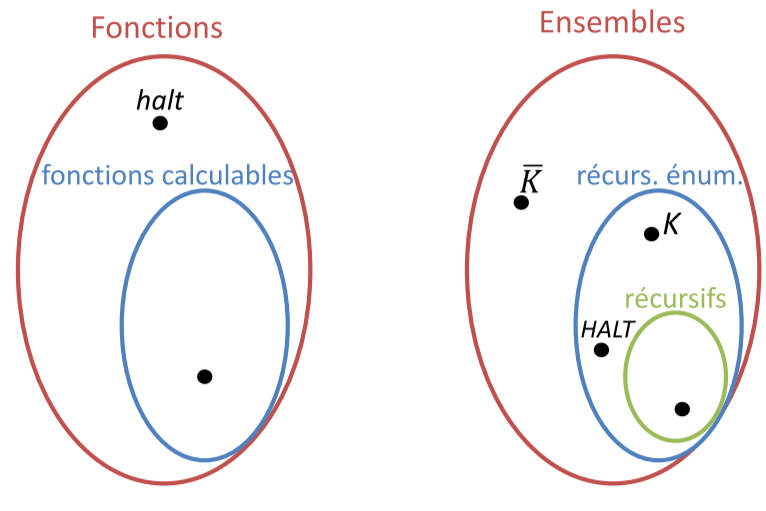
\includegraphics[width=5cm]{img/ensembleFonction.png}
\caption{Schématisation des fonctions et ensembles de fonctions}
\end{figure}

Le fait de ne pas pouvoir calculer "halt" nous pose soucis et va ouvrir tout un pan de soucis et limitations.

\section{Insuffisance des fonctions totales}
Pourquoi est-ce utile d'avoir un programme qui tourne en \textit{boucle}? N'avons-nous pas besoin de fonctions qui donnent un résultat précis tout le temps donc \textit{totale}?

Imaginons que nous créons un \textit{langage de programmation} qui a que des fonctions totales.
Donc, \textbf{Halt} est calculable et on a une réponse pour toutes fonctions. Halt serait la fonction constante 1.

Notre langage \textit{Q} est calculable donc ayant un interpréteur calculable.

\subsection{Théorème de Hoare-Allison}
Donc en résumé de notre langage \textit{Q}:
\begin{itemize}
\item L'interpréteur de ce programme est calculable
\item La fonction \textit{halt} est totale et correspond à la fonction constante de 1.
\item Mais l'interpréteur \textcolor{red}{n'est pas} calculable \textit{dans Q}.
\end{itemize}

\begin{center}
\begin{tabular}{|c|c|c|c|c|c|}
\hline
& $0$ & $1$ & ... & $k$& ...\\
\hline
$Q_0$ & \textcolor{red}{interpret(0,0)} & interpret(0,1) & ... & interpret(0,k) & ...\\
\hline
$Q_1$ & interpret(1,0) & \textcolor{red}{interpret(1,1)} & ... & interpret(1,k) & ...\\
\hline
... & ... & ... & ... & ... & ... \\
\hline
$Q_k$ & interpret(k,0) & interpret(k,1) & ... & \textcolor{red}{interpret(k,k)} & ...\\
\hline
... & ... & ... & ... & ... & ... \\
\hline
\end{tabular}
\end{center}
La colonne \textit{Q} correspond à l'ensemble des programmes et la ligne de nombre correspond aux entrées de chaque programme.

Tous les programmes se terminent donc \textit{jamais} $\perp$. On sélectionne la diagonale:
\begin{align}
diag(n) &= interpret(n,n)\\
diag_{mod}(n) &= interpret(n,n) + 1\\
Q_l &= diag_{mod}
\end{align}
Et donc, on voit facilement que à la ligne $l$ il y aura un souci avec $diag$ et notre entrée à $Q_l$ qui n'est autre que $diag_{mod}$. en effet $diag_{mod}(l) \neq diag(l)$. Donc la fonction \textit{interpret} n'est \textbf{pas} calculable en \textit{Q}.\\

Le \textit{théorème} nous dit donc que: Si un langage de programmation (non trivial) ne permet que le calcul de fonctions totales, alors: 
\begin{itemize}
\item l’interpréteur de ce langage n’est pas programmable dans ce langage 
\item il existe des fonctions totales non programmables dans ce langage
\item ce langage est \textcolor{red}{restrictif}
\end{itemize}

Donc si on peut faire un interpréteur d'un langage dans son langage, la fonction \textit{halt} n'est pas totale. Donc c'est soit programmable par lui-même soit fonction totale de halt.\\

Si on veut qu’un langage de programmation permette la programmation de toutes les fonctions totales calculables, alors ce langage doit également permettre
la programmation de fonctions non totales.\\

De plus, si on avait une fonction qui regarde si des fonctions sont totales, cela pose problème. Cela est impossible et donc cette fonction $tot(n)$ n'est pas récursif.

\subsection{Interpréteur}
Pour qu'un formalisme soit assez puissant, il faut que ce dernier arrive à programmer son propre interpréteur.

\begin{equation}
\exists z \forall n,x : \varphi_z(n,x) = \varphi_n(x)
\end{equation}
Avec $\varphi_z$ qu'on appelle la fonction universelle. et $P_z$ est le programme universel. Par convention, on appelle $\theta(n,x)$ la \textcolor{red}{fonction universelle}.

\section{Extension des fonctions partielles}
Pour l'instant, nous n'avons vu que des fonctions qui soit donnent le bon résultat soit donne $\perp$ et donc boucle. On va réaliser des \textit{extensions}, c'est-à-dire que nous allons retourner la valeur correcte dans les cas possible et un message ou autre chose pour le reste des entrées.\\

Un \textit{théorème} nous dit que, \textit{Il existe une fonction partielle calculable g telle qu’aucune fonction totale calculable n’est une extension de g}.\\
Pour prouver cela, on utilise la fonction \textit{nbstep(n,x)} qui correspond au nombre d'instruction avec l'arrêt de $P_n(x)$. ($P_n(x) = \perp$)La preuve se fait pas diagonalisation comme avant (\href{http://ezcast.uclouvain.be/ezplayer/index.php?action=view_asset_bookmark&album=LINFO1123-pub&asset=2021_02_17_21h51_34s&t=224&type=cam&token=EVKUMNQV}{vidéo}).\\

%test for pre-commit


\chapter{Questions Test d'entrée}

\section{TP1}
\begin{enumerate}
\item Effectivement, il existe une bijection entre les N et les nombres impairs positifs $\rightarrow$ en somme il existe une fonction qui transforme les N en impair positif
\item J'imagine qu'il y a une bijection mais je ne vois pas quel formule passant de N aux impairs existent car c'est le propre des nombres impairs 
\item Même raisonnement que la question 1
\item La fameuse formule qui lie N et Q car Q est juste une paire de N
\item Effectivement, sachant la diagonalisation de Cantor il est simple de le prouver
\item Pour N dans N il en existe une infinité et l'ensemble d'arrivé ne change pas grand-chose car on s'intéresse au nombre de fonction.
\item Effectivement, on a un nombre fini de langage donc de mot. Cela est dû grâce à l'alphabet fini et la longueur fixe. Donc on sait énumérer
\item Question typique vu au cours. En effet comme on a une infinité et il n'existe aucune bijection depuis les naturels etc.
\item Même cardinalité = bijection, il ne peut y avoir de bijection entre un ensemble non énumérable et énumérable
\item Une infinité de nombre mais effectivement même cardinalité car tous peuvent être ramené aux naturels.


\end{enumerate}

\section{TP2}
\begin{enumerate}
\item Effectivement, on ne doit pas être en capacité de coder l'algorithme pour que la fonction soit calculable.
\item Nombre premier est récursif car on a le crible d'eratosthène.
\item Si un ensemble $\textbf{X}$ est récursif (donc donne 1 ou 0) alors $\bar{X}$ l'est également car il inverse les 1 et 0.
\item Si $\textbf{X}$ est récursivement énumérable (donne 1 ou quelque chose d'autre mais pas 1) et que son opposé $\bar{X}$ est récursivement énumérable. Alors bien évidemment $\textbf{X}$ est récursif.
\item Oui, trivial.
\item Non, juste au simple fait que si $\textbf{X}$ est récursivement énumérable alors $\bar{X}$ ne peut être récursivement énumérable.
\item Vrai car on a une fonction calculable car ce sont des combinaisons linéaires de calculables.
\item Voir sous-section \ref{caract}.
\item Oui car être énumérable c'est dire qu'on peut compter tous les résultats même si ça prend un temps infini.
\item Voir sous-section \ref{caract}.
\end{enumerate}

\end{document}
